% $Id: slides.tex,v 1.5 2006/04/10 14:22:04 jschauma Exp $
\special{! TeXDict begin /landplus90{true}store end }

\documentclass[xga]{xdvislides}
\usepackage[landscape]{geometry}
\usepackage{graphics}
\usepackage{graphicx}
\usepackage{colordvi}
\usepackage{multirow}
\usepackage[normalem]{ulem}

\begin{document}
\setfontphv

%%% Headers and footers
\lhead{\slidetitle}                               % default:\lhead{\slidetitle}
\chead{CS615 - Aspects of System Administration}% default:\chead{\relax}
\rhead{Slide \thepage}                       % default:\rhead{\sectiontitle}
\lfoot{\Gray{Backup, Monitoring}}% default:\lfoot{\slideauthor}
\cfoot{\relax}                               % default:\cfoot{\relax}
\rfoot{\Gray{\today}}

\newcommand{\smallish}{\fontsize{16}{16}\selectfont}

\vspace*{\fill}
\begin{center}
	\Hugesize
		CS615 - Aspects of System Administration\\ [1em]
		Backup, Monitoring\\ [1em]
	\hspace*{5mm}\blueline\\ [1em]
	\Normalsize
		Department of Computer Science\\
		Stevens Institute of Technology\\
		Jan Schaumann\\
		\verb+jschauma@stevens.edu+\\
		\verb+https://www.cs.stevens.edu/~jschauma/615/+
\end{center}
\vspace*{\fill}

\subsection{"The website is down..."}
\begin{center}
	
\includegraphics[scale=0.55]{pics/monkey.eps}
\end{center}

\subsection{"The website is down..."}

\begin{verbatim}
$ curl -I https://www.cs.stevens-tech.edu/~jschauma/615/
curl: (51) SSL: no alternative certificate subject name matches
        target host name 'www.cs.stevens-tech.edu'
\end{verbatim}

\subsection{"The website is down..."}

\begin{verbatim}
$ curl -I https://www.cs.stevens.edu/~jschauma
HTTP/1.1 301 Moved Permanently
Date: Sat, 31 Mar 2018 21:09:57 GMT
Server: Apache
Location: https://www.stevens.edu/ses/cs/errors/404.html
Vary: Accept-Encoding
Content-Type: text/html; charset=iso-8859-1

$ curl -I https://www.stevens.edu/ses/cs/errors/404.html
HTTP/2 404
[...]
\end{verbatim}

\subsection{"The website is down..."}

\begin{verbatim}
$ curl -I https://www.cs.stevens.edu/~jschauma
HTTP/1.1 301 Moved Permanently
Date: Sat, 31 Mar 2018 21:09:57 GMT
Server: Apache
Location: https://www.stevens.edu/ses/cs/errors/404.html
Vary: Accept-Encoding
Content-Type: text/html; charset=iso-8859-1

$ curl -I https://www.stevens.edu/ses/cs/errors/404.html
HTTP/2 404
[...]

$ ssh jschauma@git.srcit.stevens-tech.edu
jschauma@git.srcit.stevens-tech.edu's password:
\end{verbatim}


\subsection{"The website is back up... ish"}

\begin{verbatim}
$ curl -I https://www.cs.stevens.edu/~jschauma/615/
HTTP/1.1 200 OK
Date: Sat, 31 Mar 2018 21:21:39 GMT
Server: Apache
Last-Modified: Tue, 25 Apr 2017 16:38:05 GMT
\end{verbatim}

\subsection{Backups vs. Restores}
\Huge
\begin{center}

Backups are just a {\em means} to accomplish a specific
{\em goal}: \\

\vspace{.5in}

{\bf To have the ability to restore data.}
\end{center}
\Normalsize

\subsection{To the backups!}
\vspace*{\fill}
\begin{center}
	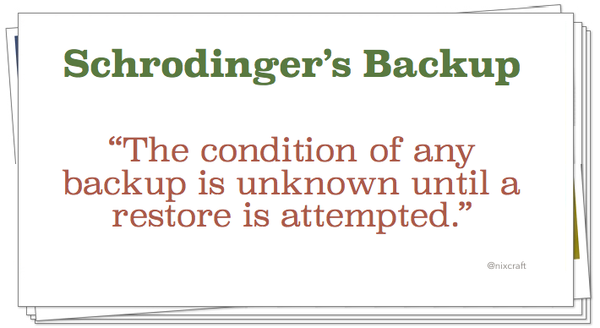
\includegraphics[scale=0.8]{pics/schrodinger.eps}
\end{center}
\vspace*{\fill}

\subsection{Backups and Restore Basics}
When do we need backups?
\begin{itemize}
	\item long-term storage / archival
	\item recover from data loss
\end{itemize}

\subsection{Long-term storage}
\vspace*{\fill}
\begin{center}
	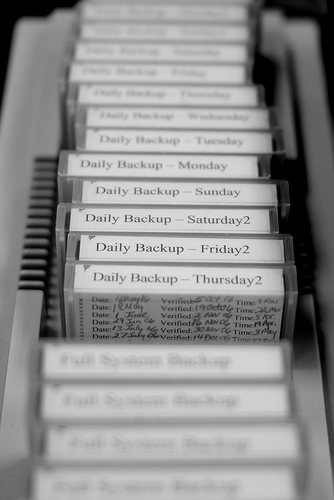
\includegraphics[scale=2.0]{pics/daily-tapes.eps}
\end{center}
\vspace*{\fill}

\subsection{Long-term storage}
\vspace*{\fill}
\begin{center}
	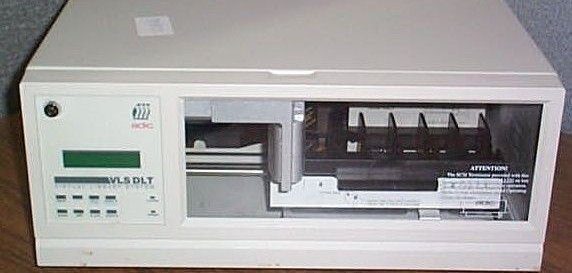
\includegraphics[scale=0.8]{pics/dlt-library.eps}
\end{center}
\vspace*{\fill}

\subsection{Long-term storage}
\vspace*{\fill}
\begin{center}
	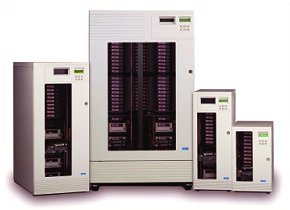
\includegraphics[scale=1.0]{pics/libraries.eps}
\end{center}
\vspace*{\fill}

\subsection{Long-term storage}
\begin{itemize}
	\item {\em full} set of level 0 backups
	\item separate set from regular backups
	\item usually stored off-site
	\item recovery / retrieval takes time
	\item limited granularity
	\item storage media considerations
	\item storage media transport considerations
	\item backup encryption and recovery key management
\end{itemize}


\subsection{Backups and Restore Basics}
When do we need backups?
\begin{itemize}
	\item long-term storage / archival
	\item recover from data loss due to
\end{itemize}
\vspace*{\fill}
\begin{center}
	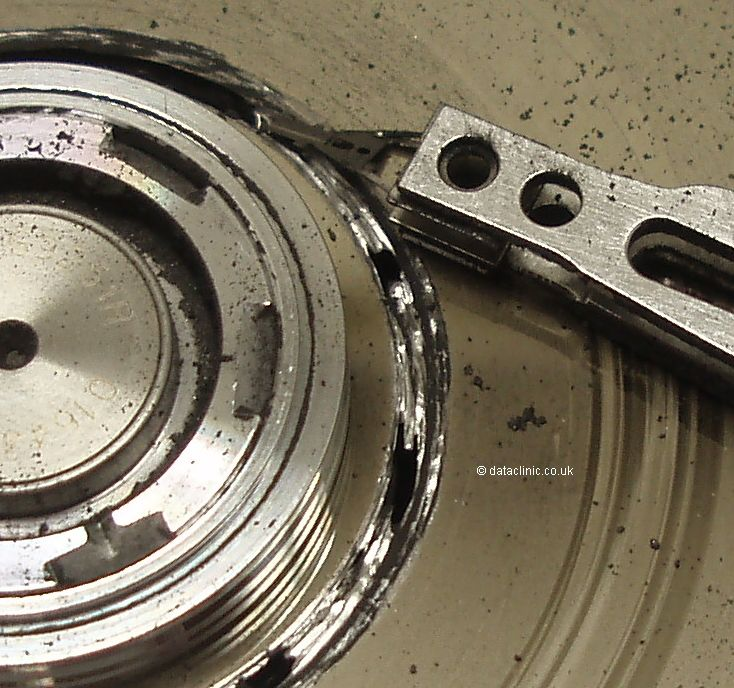
\includegraphics[scale=1.0]{pics/headcrash-closeup.eps}
\end{center}
\vspace*{\fill}

\subsection{Backups and Restore Basics}
When do we need backups?
\begin{itemize}
	\item long-term storage / archival
	\item recover from data loss due to
\end{itemize}
\vspace*{\fill}
\begin{center}
	
\includegraphics[scale=1.2]{pics/dumb-user.eps}
\end{center}
\vspace*{\fill}

\subsection{Backups and Restore Basics}
When do we need backups?
\begin{itemize}
	\item long-term storage / archival
	\item recover from data loss due to
\end{itemize}
\vspace*{\fill}
\begin{center}
	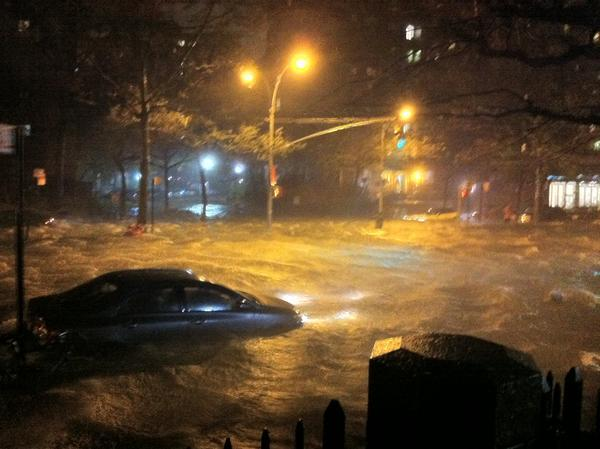
\includegraphics[scale=0.4]{pics/20th-and-C.eps}
\end{center}
\vspace*{\fill}

\subsection{Backups and Restore Basics}
When do we need backups?
\begin{itemize}
	\item long-term storage / archival
	\item recover from data loss due to
\end{itemize}
\vspace*{\fill}
\begin{center}
	
\includegraphics[scale=0.6]{pics/hacker.eps}
\end{center}
\vspace*{\fill}

\subsection{Backups and Restore Basics}
When do we need backups?
\begin{itemize}
	\item long-term storage / archival
	\item recover from data loss due to
\end{itemize}
\vspace*{\fill}
\begin{center}
	
\includegraphics[scale=0.6]{pics/bugs.eps}
\end{center}
\vspace*{\fill}

\subsection{Backups and Restore Basics}
When do we need backups?
\begin{itemize}
	\item long-term storage / archival
	\item recover from data loss due to
		\begin{itemize}
			\item equipment failure
			\item bozotic users
			\item natural disaster
			\item security breach
			\item software bugs
		\end{itemize}
\end{itemize}

\subsection{Backups and Restore Basics}
When do we need backups?
\begin{itemize}
	\item long-term storage / archival
	\item recover from data loss due to
		\begin{itemize}
			\item equipment failure
			\item bozotic users
			\item natural disaster
			\item security breach
			\item software bugs
		\end{itemize}
\end{itemize}
\addvspace{.5in}
Think of your backups as {\em insurance}:  you invest and pay for it, hoping
you will never need it.

\subsection{Disaster Recovery}
\begin{itemize}
	\item loss of e.g. entire file system
	\item leads to downtime (of individual systems)
	\item RAID may help
	\item takes long time to restore
	\item may require retrieval of archival backups from long-term storage 
	\item often involves {\em some} data loss
\end{itemize}

\subsection{Disaster Recovery}
\begin{itemize}
	\item loss of e.g. entire file system
	\item leads to downtime (of individual systems)
	\item RAID may help
	\item takes long time to restore
	\item may require retrieval of archival backups from long-term storage 
	\item often involves {\em some} data loss
\end{itemize}
\vspace{.5in}
Beware: disasters scale up much faster than your
backup strategy!

\subsection{File deletion recovery}
Accidentally deleted files ought to be recoverable for
a certain amount of time:
\begin{itemize}
	\item "Undo"
	\item time window and granularity requirements
	\item restore time, including
		\begin{itemize}
			\item actual time spent restoring
			\item waiting until resources permit the restore
			\item staff availability
		\end{itemize}
	\item self-service restore
\end{itemize}
\vspace{.5in}
But note: sometimes people {\em do} want to delete
data and it be gone!

% \subsection{Filesystem backup}
% \begin{itemize}
% 	\item start an EC2 instance
% 	\item create a full filesystem backup using \verb+dump(8)+
% 	\item add e.g. the 'apache' package
% 	\item create an incremental backup
% 	\item delete the 'apache' package
% 	\item restore all files from the incremental backup using the \verb+restore(8)+ command
% 	\item verify that the 'apache' package is fully installed
% \end{itemize}
 
\subsection{Filesystem backup}
\smallish
\begin{verbatim}
ssh ec2-instance "dump -u -0 -f - /" | bzip2 -c -9 >tmp/ec2.0.bz2
  DUMP: Found /dev/rxbd1a on / in /etc/fstab
  DUMP: Date of this level 0 dump: Mon Apr  2 19:34:30 2018
  DUMP: Date of last level 0 dump: the epoch
  DUMP: Dumping /dev/rxbd1a (/) to standard output
  DUMP: Label: none
  DUMP: mapping (Pass I) [regular files]
  DUMP: mapping (Pass II) [directories]
  DUMP: estimated 962609 tape blocks.
  DUMP: Volume 1 started at: Mon Apr  2 19:34:34 2018
  DUMP: dumping (Pass III) [directories]
  DUMP: dumping (Pass IV) [regular files]
  DUMP: 42.40% done, finished in 0:06
  DUMP: 83.38% done, finished in 0:01
  DUMP: 963445 tape blocks
  DUMP: Volume 1 completed at: Mon Apr  2 19:46:38 2018
  DUMP: Volume 1 took 0:12:04
  DUMP: Volume 1 transfer rate: 1330 KB/s
  DUMP: Date of this level 0 dump: Mon Apr  2 19:34:30 2018
  DUMP: Date this dump completed:  Mon Apr  2 19:46:38 2018
  DUMP: Average transfer rate: 1330 KB/s
  DUMP: level 0 dump on Mon Apr  2 19:34:30 2018
  DUMP: DUMP IS DONE
\end{verbatim}
\Normalsize


\subsection{Filesystem backup}
\smallish
\begin{verbatim}
$ cat /etc/dumpdates
/dev/rxbd1a      0 Mon Apr  2 19:34:30 2018
$ ssh ec2-instance "dump -u -i -f - /" | bzip2 -c -9 >tmp/ec2.1.bz2
  DUMP: Found /dev/rxbd1a on / in /etc/fstab
  DUMP: Date of this level i dump: Mon Apr  2 20:09:24 2018
  DUMP: Date of last level 0 dump: Mon Apr  2 19:34:30 2018
  DUMP: Dumping /dev/rxbd1a (/) to standard output
  DUMP: Label: none
  DUMP: mapping (Pass I) [regular files]
  DUMP: mapping (Pass II) [directories]
  DUMP: estimated 25307 tape blocks.
  DUMP: Volume 1 started at: Mon Apr  2 20:09:33 2018
  DUMP: dumping (Pass III) [directories]
  DUMP: dumping (Pass IV) [regular files]
  DUMP: 25244 tape blocks
  DUMP: Volume 1 completed at: Mon Apr  2 20:09:50 2018
  DUMP: Volume 1 took 0:00:17
  DUMP: Volume 1 transfer rate: 1484 KB/s
  DUMP: Date of this level i dump: Mon Apr  2 20:09:24 2018
  DUMP: Date this dump completed:  Mon Apr  2 20:09:50 2018
  DUMP: Average transfer rate: 1484 KB/s
  DUMP: level i dump on Mon Apr  2 20:09:24 2018
  DUMP: DUMP IS DONE
\end{verbatim}
\Normalsize

\subsection{Filesystem backup}
\smallish
\begin{verbatim}
$ rm /etc/resolv.conf # oops
$ restore -i -f /backups/ec2.0
...
\end{verbatim}

\subsection{Poor Man's Cloud Backup via {\tt tar(1)}}
Copying to a file system:
\begin{verbatim}
$ tar cf - data/ | ssh ec2-instance "tar -xf - -C /var/backups/$(date)"
\end{verbatim}

\vspace{.5in}
Writing to a block device, no filesystem necessary:
\begin{verbatim}
$ tar cf - data/ | ssh ec2-instance "dd of=/dev/rxb2a"
$ ssh ec2-instance "dd if=/dev/rxb2a" | tar tvf -
\end{verbatim}

\vspace{.5in}
Encrypting along the way:
\begin{verbatim}
$ tar cf - data/ | gpg --encrypt -r recipient | ssh ec2-instance "dd of=/dev/rxb2a"
\end{verbatim}

\subsection{Know a Unix Command}
\vspace*{\fill}
\begin{center}
	
\includegraphics[scale=0.9]{pics/tar.eps} \\
	\verb+https://www.xkcd.com/1168/+ \\
	\verb+https://www.cs.stevens.edu/~jschauma/615/tar.html+
\end{center}
\vspace*{\fill}

\subsection{Filesystem backup}
\vspace*{\fill}
\begin{center}
	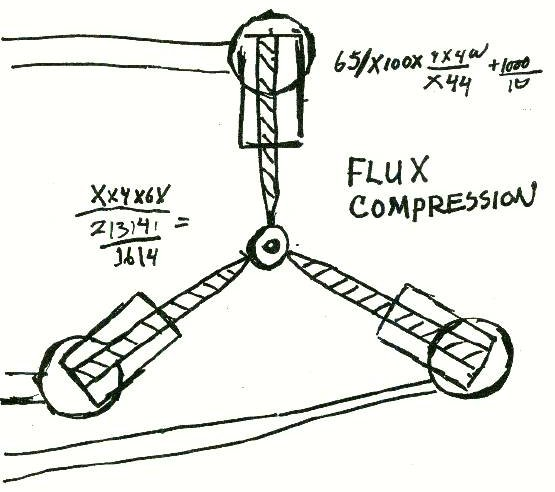
\includegraphics[scale=0.7]{pics/flux-capacitor.eps}
\end{center}
\vspace*{\fill}

\subsection{Filesystem backup}
\vspace*{\fill}
\begin{center}
	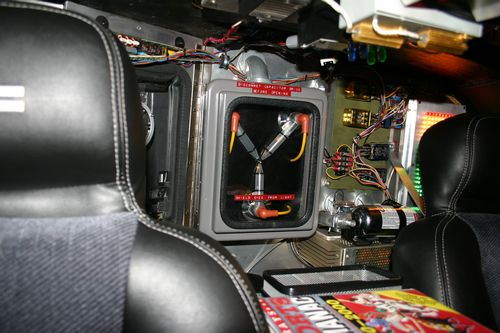
\includegraphics[scale=2.5]{pics/flux-capacitor2.eps}
\end{center}
\vspace*{\fill}

\subsection{Filesystem backup}
\vspace*{\fill}
\begin{center}
	
\includegraphics[scale=0.6]{pics/Time_Machine.eps}
\end{center}
\vspace*{\fill}


\subsection{Filesystem backup}
Example: Mac OS X ``Time Machine'':
\begin{itemize}
	\item automatically creates a full backup (equivalent of a "level 0 dump")
		to separate device or NAS, recording (specifically) last-modified date
		of all directories
	\item every hour, creates a full copy via {\em hardlinks} (hence no
		additional disk space consumed) for files that have not changed,
		new copy of files that have changed
		\item changed files are determined by inspecting last-modified date of
			directories (cheaper than doing comparison of all files'
			last-modified date or data)
	\item saves hourly backups for 24 hours, daily backups for
		the past month, and weekly backups for everything older than a month.
\end{itemize}

\subsection{Filesystem backup}
Example: WAFL (Write Anywhere File Layout)
\begin{itemize}
	\item used by NetApp's ``Data ONTAP'' OS
	\item a snapshot is a read-only copy of a file system (cheap and near
		instantaneous, due to CoW)
	\item uses regular snapshots (``consistency points'', every 10 seconds)
		to allow for speedy recovery from crashes
\end{itemize}
\vspace*{\fill}
\begin{center}
	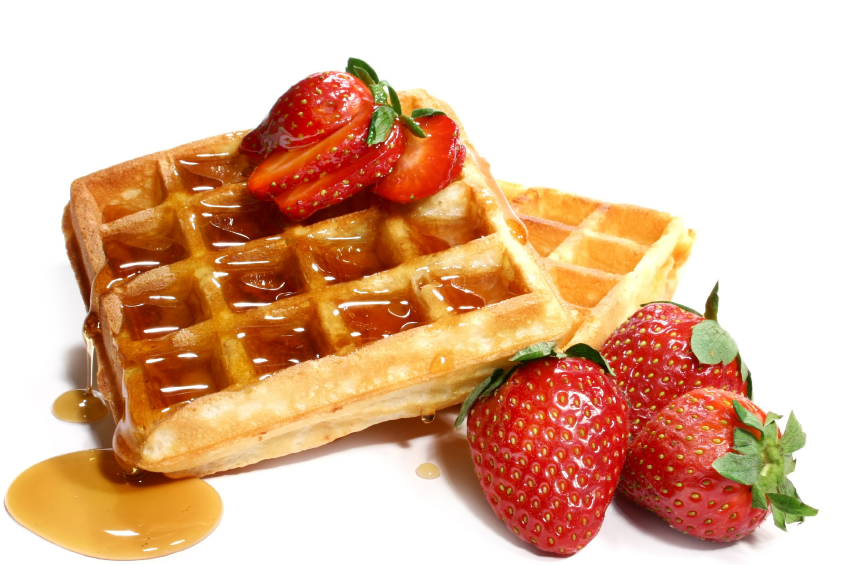
\includegraphics[scale=0.75]{pics/waffles.eps}
\end{center}
\vspace*{\fill}


\subsection{Filesystem backup}
Example: WAFL (Write Anywhere File Layout)
\vspace*{\fill}
\begin{center}
	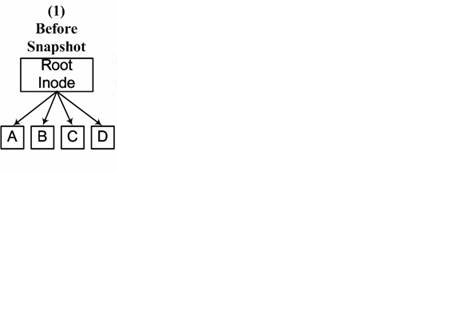
\includegraphics[scale=1.0]{pics/wafl0.eps}
\end{center}
\vspace*{\fill}


\subsection{Filesystem backup}
Example: WAFL (Write Anywhere File Layout)
\vspace*{\fill}
\begin{center}
	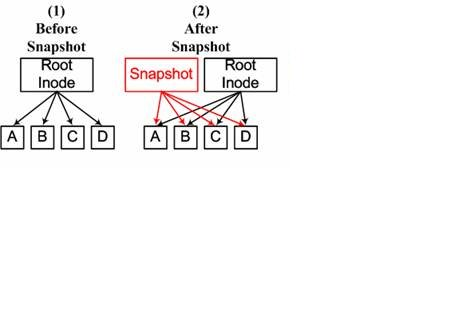
\includegraphics[scale=1.0]{pics/wafl1.eps}
\end{center}
\vspace*{\fill}


\subsection{Filesystem backup}
Example: WAFL (Write Anywhere File Layout)
\vspace*{\fill}
\begin{center}
	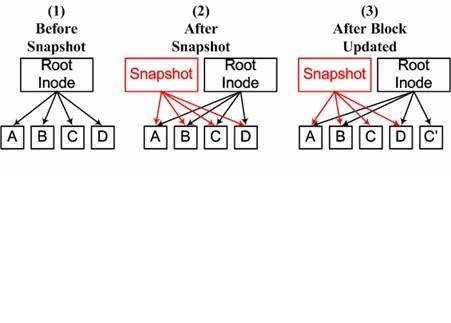
\includegraphics[scale=1.0]{pics/wafl2.eps}
\end{center}
\vspace*{\fill}


\subsection{Filesystem backup}
Example: WAFL (Write Anywhere File Layout)
\vspace*{\fill}
\begin{center}
	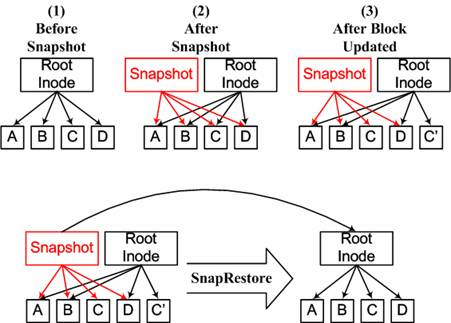
\includegraphics[scale=1.0]{pics/wafl.eps}
\end{center}
\vspace*{\fill}


\subsection{Filesystem backup}
Example: ZFS snapshots
\begin{itemize}
	\item ZFS uses a copy-on-write transactional object model (new data does
		not overwrite existing data, instead modifications are written to a
		new location with existing data being referenced), similar to WAFL
	\item a snapshot is a read-only copy of a file system (cheap and near
		instantaneous, due to CoW)
	\item initially consumes no additional disk space; the writable filesystem
		is made available as a ``clone''
	\item conceptually provides a branched view of the filesystem; normally
		only the ``active'' filesystem is writable
\end{itemize}

\subsection{ZFS Snapshots}
\smallish
\begin{verbatim}
$ pwd
/home/jschauma
$ ls -l .z*
ls: cannot access .z*: No such file or directory
$
\end{verbatim}
\Normalsize

\subsection{ZFS Snapshots}
\smallish
\begin{verbatim}
$ pwd
/home/jschauma
$ ls -l .z*
ls: cannot access .z*: No such file or directory
$ ls -lid .zfs
1 dr-xr-xr-x 3 root root 3 Jan 10  2013 .zfs
$
\end{verbatim}
\Normalsize

\subsection{ZFS Snapshots}
\smallish
\begin{verbatim}
$ pwd
/home/jschauma
$ ls -l .z*
ls: cannot access .z*: No such file or directory
$ ls -lid .zfs
1 dr-xr-xr-x 3 root root 3 Jan 10  2013 .zfs
$ ls -lai .zfs/snapshot
total 13
2 dr-xr-xr-x  4 root     root       4 Feb 28 21:00 .
1 dr-xr-xr-x  3 root     root       3 Jan 10  2013 ..
4 drwx--x--x 37 jschauma professor 88 Feb 24 22:32 amanda-_export_home_jschauma-0
4 drwx--x--x 37 jschauma professor 88 Feb 26 11:47 amanda-_export_home_jschauma-1
$
\end{verbatim}
\Normalsize

\subsection{ZFS Snapshots}
\smallish
\begin{verbatim}
$ pwd
/home/jschauma
$ ls -l .z*
ls: cannot access .z*: No such file or directory
$ ls -lid .zfs
1 dr-xr-xr-x 3 root root 3 Jan 10  2013 .zfs
$ ls -lai .zfs/snapshot
total 13
2 dr-xr-xr-x  4 root     root       4 Feb 28 21:00 .
1 dr-xr-xr-x  3 root     root       3 Jan 10  2013 ..
4 drwx--x--x 37 jschauma professor 88 Feb 24 22:32 amanda-_export_home_jschauma-0
4 drwx--x--x 37 jschauma professor 88 Feb 26 11:47 amanda-_export_home_jschauma-1
$ cd .zfs/snapshot
$ echo foo > amanda-_export_home_jschauma-0/oink
-ksh: amanda-_export_home_jschauma-0/oink: cannot create [Read-only file system]
$ ls -laid . /
2 dr-xr-xr-x  4 root root    4 Feb 28 21:00 .
2 drwxr-xr-x 26 root root 4096 Jan 27 11:44 /
\end{verbatim}
\Normalsize

\subsection{ZFS Snapshots}
\smallish
\begin{verbatim}
$ pwd
/home/jschauma/.zfs/snapshot
$ ls -lai amanda-_export_home_jschauma-0 >/tmp/a
$ ls -lai amanda-_export_home_jschauma-1 >/tmp/b
$ diff -bu /tmp/[ab]
--- /tmp/a	2014-03-01 22:55:49.000000000 -0500
+++ /tmp/b	2014-03-01 22:55:59.000000000 -0500
@@ -35,7 +35,7 @@
 57723 drwx------  3 jschauma professor         6 Dec 31 15:08 .subversion
 49431 -rw-------  1 jschauma professor         6 Dec 22 12:25 .sws.pid
    20 drwx------  2 jschauma professor         3 Jan 26 10:30 .vim
-61768 -rw-------  1 jschauma professor     14538 Feb 24 22:32 .viminfo
+61775 -rw-------  1 jschauma professor     14557 Feb 26 09:23 .viminfo
   173 -rw-------  1 jschauma professor      4355 Sep 17  2012 .vimrc
 45744 -rw-r--r--  1 jschauma professor         0 Jul 28  2013 .xsession-errors
    21 drwxr-xr-x  3 jschauma professor         6 Apr  4  2010 CS615A
$
\end{verbatim}
\Normalsize

\subsection{Summary}
\begin{itemize}
	\item backups are most commonly done as incrementals
		of a filesystem, mountpoint, or directory hierarchy
	\item consider (long-term) storage:
		\begin{itemize}
			\item media and location
			\item increased storage requirements
			\item privacy and safety of the data
		\end{itemize}
	\item self-service restores and filesystem snapshots
	\item backups need to be:
		\begin{itemize}
			\item regular, frequent, automated
			\item invisible
			\item verifiable
			\item regularly tested
		\end{itemize}
\end{itemize}

\newpage
\vspace*{\fill}
\begin{center}
	\Hugesize
		Hooray!\\ [1em]
	\hspace*{5mm}
	\blueline\\
	\hspace*{5mm}\\
		5 minute break
\end{center}
\vspace*{\fill}


\subsection{Problem Report}
\vspace*{\fill}
\Huge
\begin{center}
``Something's wrong.''
\end{center}
\Normalsize
\vspace*{\fill}

\subsection{Now what?}
\begin{center}
	
\includegraphics[scale=0.55]{pics/monkey.eps}
\end{center}

\subsection{Problem Report}
\vspace*{\fill}
\Huge
\begin{center}
``The system feels slow.'' \\
\addvspace{.5in}
``I can't log in.'' \\
\addvspace{.5in}
``My mail was not delivered.'' \\
\addvspace{.5in}
``The site is down.''
\end{center}
\Normalsize
\vspace*{\fill}

\subsection{Now what?}
\begin{center}
	
\includegraphics[scale=0.55]{pics/monkey.eps}
\end{center}

\subsection{To the logs!}
\begin{center}
	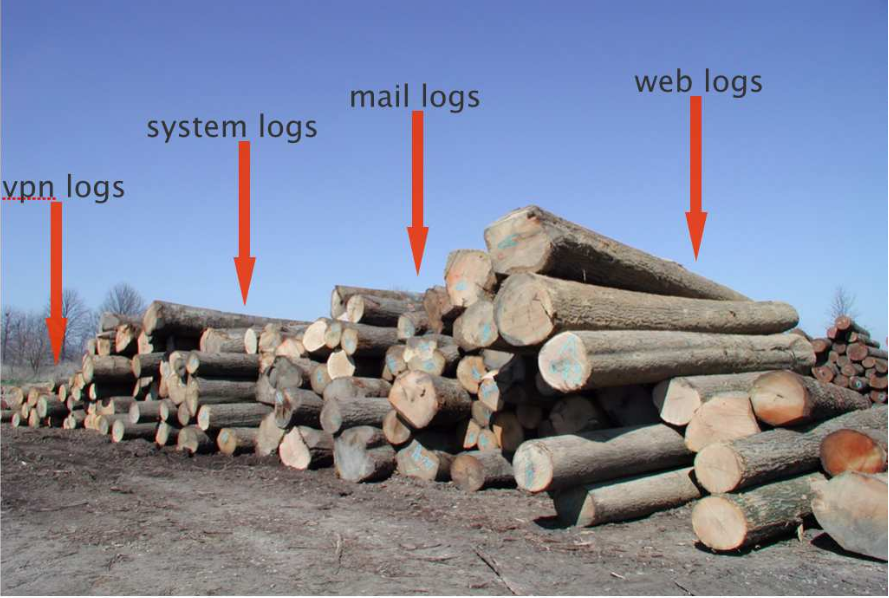
\includegraphics[scale=0.55]{pics/logs.eps}
\end{center}

\subsection{Answers}
``The system feels slow.''
\begin{verbatim}
up 1318 days, 13:46, 1 user, load averages: 993.81, 272.91, 1012.18
\end{verbatim}

\addvspace{.3in}
``I can't log in.''
\begin{verbatim}
Apr 6 09:25:56 <auth.info>hostname sshd[1624]: Failed password for jdoe from
115.239.231.100 port 1047 ssh2
\end{verbatim}

\addvspace{.3in}
``My mail was not delivered.''
\begin{verbatim}
Apr 11 16:15:40 panix postfix/smtpd[7566]: connect from unknown[122.3.68.122]
Apr 11 16:15:41 panix postfix/smtpd[7566]: NOQUEUE: reject_warning: RCPT from
unknown[122.3.68.122]: 450 4.7.1 Client host rejected: cannot find your hostname,
[122.3.68.122]; from=<McneilRomany28@pldt.net> to=<jschauma@stevens.edu>
proto=ESMTP helo=<122.3.68.122.pldt.net>
\end{verbatim}

\subsection{Answers}
``The site is down.'' \\

\begin{verbatim}
94.242.252.41 - "" [11/Apr/2016:19:18:47 -0400] "GET /secret/ HTTP/1.1"
403 524 "-" "Mozilla/5.0 (Macintosh; Intel Mac OS X 10.9; rv:28.0)
Gecko/20100101 Firefox/28.0"
\end{verbatim}

\subsection{Answers}
``The site is down.'' \\

\begin{verbatim}
94.242.252.41 - "" [11/Apr/2016:19:18:47 -0400] "GET /secret/ HTTP/1.1"
403 524 "-" "Mozilla/5.0 (Macintosh; Intel Mac OS X 10.9; rv:28.0)
Gecko/20100101 Firefox/28.0"
\end{verbatim}

\addvspace{.2in}
\begin{center}
	
\includegraphics[scale=0.25]{pics/monkey.eps}
\end{center}

\subsection{Events}
\vspace*{\fill}
\Huge
\begin{center}
``Something's wrong.'' is just an {\em unexpected} or
{\em undesirable} event.
\end{center}
\Normalsize
\vspace*{\fill}

\subsection{Events}
\vspace*{\fill}
\Huge
\begin{center}
``Something's wrong.'' is just an {\em unexpected} or
{\em undesirable} event. \\
\vspace{.4in}
{\em Events} happen all the time.
\end{center}
\Normalsize
\vspace*{\fill}

\subsection{Events}
\vspace*{\fill}
\Huge
\begin{center}
``Something's wrong.'' is just an {\em unexpected} or
{\em undesirable} event. \\
\vspace{.4in}
{\em Events} happen all the time. \\
\vspace{.4in}
Being able to identify {\em relevant} events allows
you to diagnose, predict and even prevent {\em
undesirable} events.
\end{center}
\Normalsize
\vspace*{\fill}

\subsection{Events}
\vspace*{\fill}
\Huge
\begin{center}
In order to be able to identify an event as {\em
unexpected}, you have to have {\em expected} events.
\end{center}
\Normalsize
\vspace*{\fill}

\subsection{Expected Events}
\vspace*{\fill}
\Huge
\begin{center}
Know your applications.
\end{center}
\Normalsize
\vspace*{\fill}

\subsection{Expected Events}
\vspace*{\fill}
\Huge
\begin{center}
Know your applications. \\
\vspace{.4in}
Know your users.
\end{center}
\Normalsize
\vspace*{\fill}

\subsection{Expected Events}
\vspace*{\fill}
\Huge
\begin{center}
Know your applications. \\
\vspace{.4in}
Know your users. \\
\vspace{.4in}
Know your traffic patterns.
\end{center}
\Normalsize
\vspace*{\fill}

\subsection{Expected Events}
\vspace*{\fill}
\Huge
\begin{center}
Know your applications. \\
\vspace{.4in}
Know your users. \\
\vspace{.4in}
Know your traffic patterns. \\
\vspace{.4in}
{\em Know your systems.}
\end{center}
\Normalsize
\vspace*{\fill}

\subsection{Events and Metrics}
\vspace*{\fill}
\begin{verbatim}
$ dict event
  event
      n 1: something that happens at a given place and time
      2: a special set of circumstances; "in that event, the first
         possibility is excluded"; "it may rain in which case the
         picnic will be canceled" [syn: {event}, {case}]


$ dict metric
  metric
      3: a system of related measures that facilitates the
         quantification of some particular characteristic [syn:
         {system of measurement}, {metric}]

\end{verbatim}
\vspace*{\fill}

\subsection{Events and Metrics}
\begin{center}
	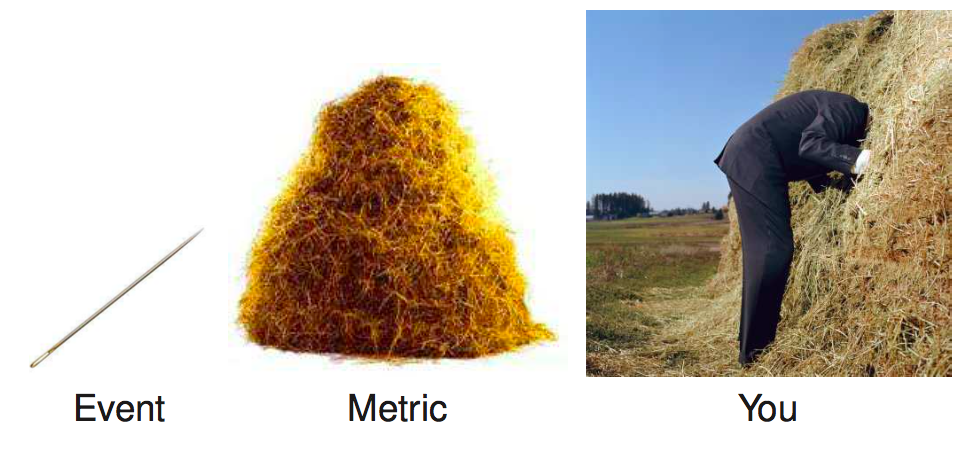
\includegraphics[scale=0.75]{pics/events-metrics.eps}
\end{center}

\subsection{Events and Metrics}
Events
\begin{itemize}
	\item may occur rarely / frequently / constantly
	\item can be collected in logs
	\item may be comprised of other events
	\item may be: ’something happened’
	\item may be: ’nothing (new) happened’
\end{itemize}
\addvspace{.5in}

Metrics:
\begin{itemize}
	\item correlation of related events
	\item may help identify outliers
	\item may trigger events
	\item may help make (automated or interactive) decisions
\end{itemize}


\subsection{Collecting Data}
{\em Counters}: easy, numeric data tracking individual events. Example: HTTP status codes

\addvspace{.5in}
{\em Timers}: easy, numeric data tracking event duration. Example: Time to send all
data for a successful HTTP request.

\addvspace{.5in}
{\em Thresholds}: easy, numeric trigger for events; may itself trigger events or metrics.
Example: more than N HTTP hits in X seconds yield 404.

% % \subsection{Counting counters, timing timers...}
% % SNMP
% % \vspace{.5in}
% % \begin{center}
% % 	\Huge
% % 	A complete network management system to monitor network-attached devices.
% % \end{center}
% % \Normalsize
% % 
% % \subsection{SNMP}
% % Base concepts:
% % \begin{itemize}
% % 	\item managed devices run an {\em snmp agent} or d\ae mon
% % 	\item information about the device is exposed in {\em management information bases}
% % 	\item parts of a system are made available in {\em read-only} mode
% % 	\item parts of a system may be made available in {\em write} mode
% % 	\item certain conditions may trigger actions or {\em traps}
% % 	\item normally uses UDP 161 for the {\em agent} and 162 for the {\em manager}
% % \end{itemize}
% % 
% % \subsection{SNMP}
% % Management Information Bases (MIBs):
% % \begin{itemize}
% % 	\item hierarchical namespace
% % 	\item contains {\em Object Identifiers} (OIDs)
% % 	\item written in {\em Abstract Syntax Notation One} (ASN.1)
% % 	\item often vendor defined
% % \end{itemize}
% % 
% % \subsection{SNMP Versions}
% % SNMPv1:
% % \begin{itemize}
% % 	\item de-facto standard
% % 	\item poor security (``community strings'' act as passwords)
% % \end{itemize}
% % \vspace{.2in}
% % SNMPv2:
% % \begin{itemize}
% % 	\item improvements in the area of performance (\verb+GETBULK+ instead of \verb+GETNEXT+) and security
% % 	\item comes in the flavors {\em SNMPv2c}, {\em SNMPv1.5} and {\em SNMPv2u}
% % \end{itemize}
% % \vspace{.2in}
% % SNMPv3:
% % \begin{itemize}
% % 	\item official standard
% % 	\item adds authentication, privacy and access control
% % \end{itemize}
% % 
% % \subsection{SNMP: An example}
% % \smallish
% % \begin{verbatim}
% % $ snmpwalk -c public -v 1 bluemoon.cs.stevens-tech.edu
% % iso.3.6.1.2.1.1.1.0 = STRING: "HP ETHERNET MULTI-ENVIRONMENT,ROM none,JETDIRECT,JD147,EEPROM
% % JDI2300 0013,CIDATE 07/13/2013"
% % iso.3.6.1.2.1.1.2.0 = OID: iso.3.6.1.4.1.11.2.3.9.1
% % iso.3.6.1.2.1.1.3.0 = Timeticks: (293219400) 33 days, 22:29:54.00
% % [...]
% % iso.3.6.1.2.1.25.3.2.1.3.1 = STRING: "HP Color LaserJet CP5520 Series"
% % iso.3.6.1.2.1.25.3.2.1.3.2 = STRING: "SanDisk SDSA5AK-008G-1006"
% % [...]
% % iso.3.6.1.2.1.43.16.5.1.2.1.1 = STRING: "Sleep mode on"
% % \end{verbatim}
% % 
% % \subsection{SNMP: An example}
% % \smallish
% % \begin{verbatim}
% % $ snmpwalk -c public -v 1 gw.cc.stevens-tech.edu
% % SNMPv2-MIB::sysDescr.0 = STRING: Cisco IOS Software, s72033_rp Software
% % (s72033_rp-ADVIPSERVICESK9_WAN-M), Version 12.2(33)SXH, RELEASE SOFTWARE (fc5)
% % DISMAN-EVENT-MIB::sysUpTimeInstance = Timeticks: (3112108803) 360 days, 4:44:48.03
% % SNMPv2-MIB::sysContact.0 = STRING: chose@stevens.edu x5457
% % SNMPv2-MIB::sysName.0 = STRING: gw.cc.stevens-tech.edu
% % SNMPv2-MIB::sysLocation.0 = STRING: campus:sl:0:machineroom
% % SNMPv2-MIB::sysORLastChange.0 = Timeticks: (0) 0:00:00.00
% % [...]
% % IF-MIB::ifPhysAddress.1 = STRING: 0:17:95:68:d2:dc
% % IF-MIB::ifPhysAddress.2 = STRING: 0:18:74:1c:e3:80
% % [...]
% % IF-MIB::ifAdminStatus.1 = INTEGER: up(1)
% % IF-MIB::ifAdminStatus.2 = INTEGER: down(2)
% % [...]
% % IF-MIB::ifInOctets.1 = Counter32: 147341347
% % IF-MIB::ifInOctets.2 = Counter32: 487894092
% % [...]
% % IF-MIB::ifOutOctets.1 = Counter32: 956876160
% % IF-MIB::ifOutOctets.2 = Counter32: 1532452749
% % [...]
% % RFC1213-MIB::ipRouteDest.66.193.255.0 = IpAddress: 66.193.255.0
% % RFC1213-MIB::ipRouteDest.66.194.0.0 = IpAddress: 66.194.0.0
% % [...]
% % \end{verbatim}
% % \Normalsize
% % 
% % \subsection{SNMP: An example}
% % \smallish
% % \begin{verbatim}
% % $ snmpwalk -Os -c public -v 1 localhost
% % iso.3.6.1.2.1.1.1.0 = STRING: "Linux avatar 3.2.0-51-generic #77-Ubuntu SMP Wed Jul 24 20:18:19
% % UTC 2013 x86_64"
% % iso.3.6.1.2.1.1.2.0 = OID: iso.3.6.1.4.1.8072.3.2.10
% % iso.3.6.1.2.1.1.3.0 = Timeticks: (31099465) 3 days, 14:23:14.65
% % [...]
% % iso.3.6.1.2.1.1.5.0 = STRING: "avatar"
% % iso.3.6.1.2.1.25.1.4.0 = STRING: "root=/dev/xvda2 ro
% % root=/dev/xvda2 ro ip=:127.0.255.255::::eth0:dhcp"
% % \end{verbatim}
% % \Normalsize

\subsection{Know Your Systems}
Profile your application:
\begin{itemize}
	\item execution time (for example: {\tt time(1)})
	\item data sources and destination affect execution
	\item {\tt strace(1)} and friends for more detailed analysis
\end{itemize}

\addvspace{.5in}
Understand your system performance:
\begin{itemize}
	\item CPU load, memory (for example: {\tt top(1)}, {\tt vmstat(1)})
	\item disk I/O (for example: {\tt iostat(1)})
	\item user activity (for example: {\tt ac(1)}, {\tt lsof(8)}, {\tt sa(8)})
\end{itemize}

\subsection{Know Your Systems}
Network statistics:
\begin{itemize}
	\item ports and applications (for example: {\tt lsof(8)}, {\tt netstat(8)})
	\item packets in and out
	\item connection origin
	\item {\em NetFlow} etc.
\end{itemize}

\subsection{Context}
{\em Context} lets you find {\em relevant} events in
your haystack of metrics.

\begin{center}
	
\includegraphics[scale=0.75]{pics/glass-needle.eps}
\end{center}

\subsection{No context.}
CPU load - 12 hours
\begin{center}
	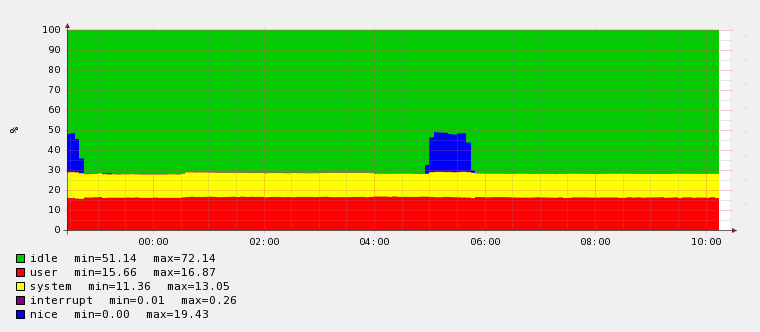
\includegraphics[scale=0.9]{pics/cpu-12h.eps}
\end{center}

\subsection{No context.}
Disk I/O - 12 hours
\begin{center}
	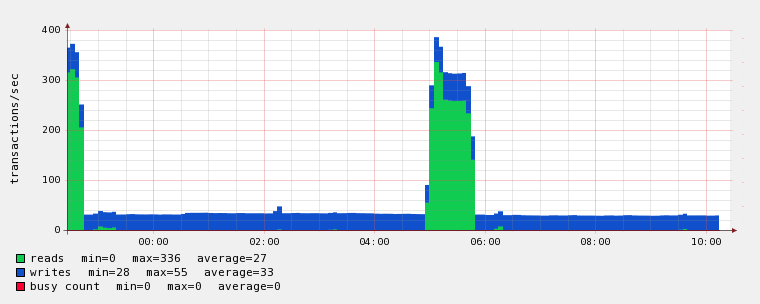
\includegraphics[scale=0.9]{pics/disk-io-12h.eps}
\end{center}

\subsection{No context.}
Load Average - 12 hours
\begin{center}
	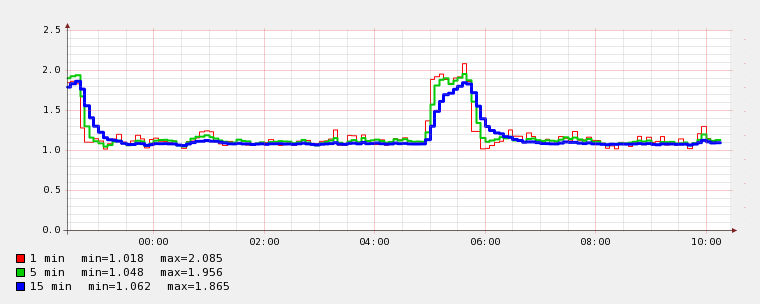
\includegraphics[scale=0.9]{pics/load-average-12h.eps}
\end{center}

\subsection{No context.}
Memory - 12 hours
\begin{center}
	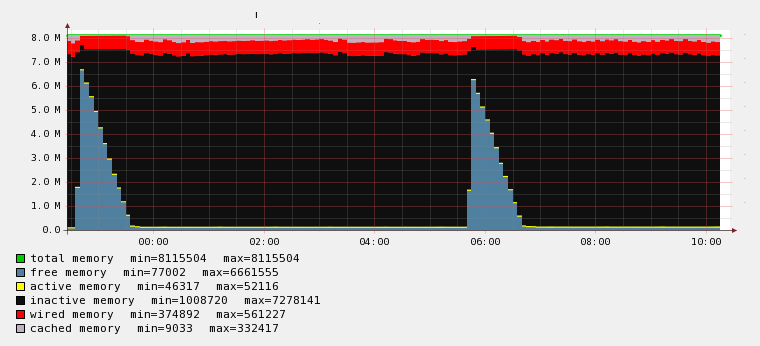
\includegraphics[scale=0.9]{pics/memory-12h.eps}
\end{center}

\subsection{Some context.}
12 hours
\begin{center}
	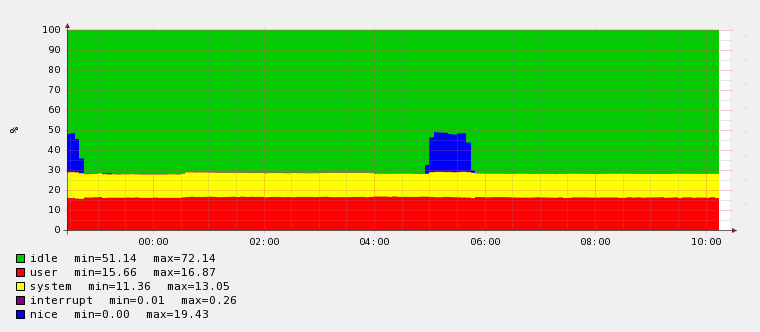
\includegraphics[scale=0.36]{pics/cpu-12h.eps}
	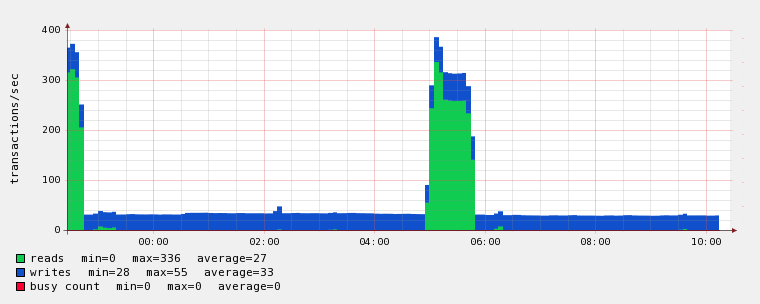
\includegraphics[scale=0.36]{pics/disk-io-12h.eps} \\
	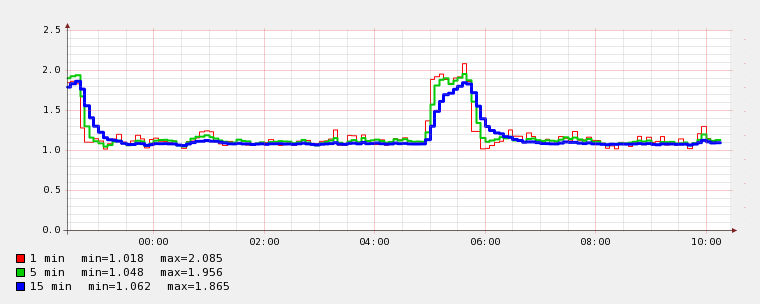
\includegraphics[scale=0.36]{pics/load-average-12h.eps}
	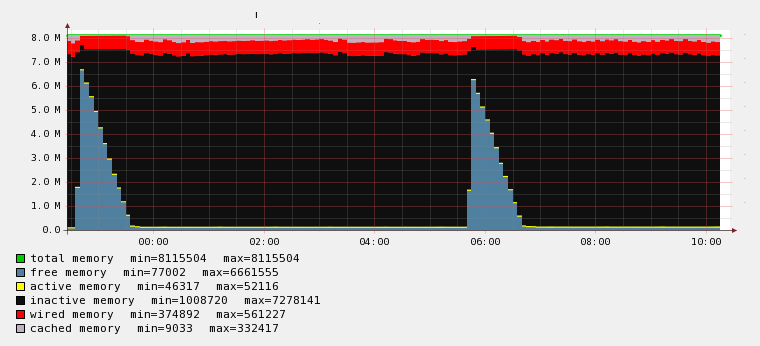
\includegraphics[scale=0.36]{pics/memory-12h.eps} \\
\end{center}

\subsection{With context.}
7 days
\begin{center}
	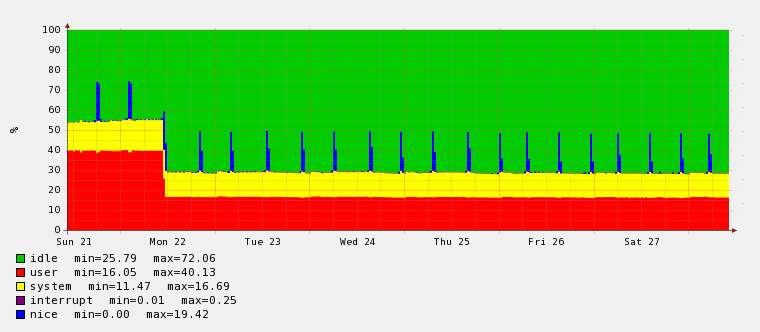
\includegraphics[scale=0.36]{pics/cpu-7day.eps}
	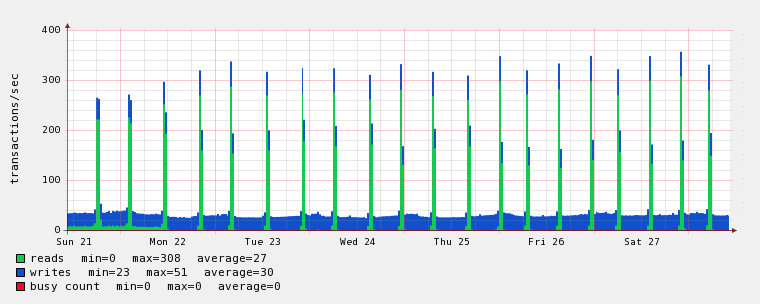
\includegraphics[scale=0.36]{pics/disk-io-7day.eps} \\
	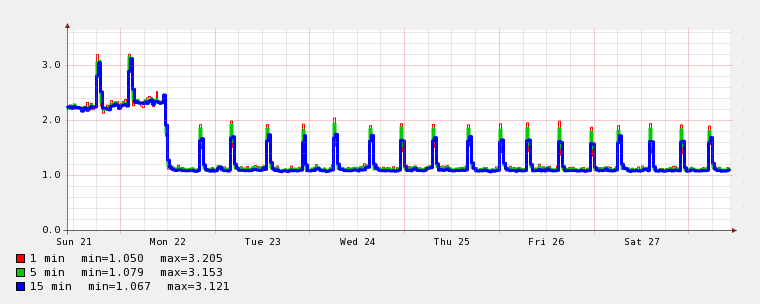
\includegraphics[scale=0.36]{pics/load-average-7day.eps}
	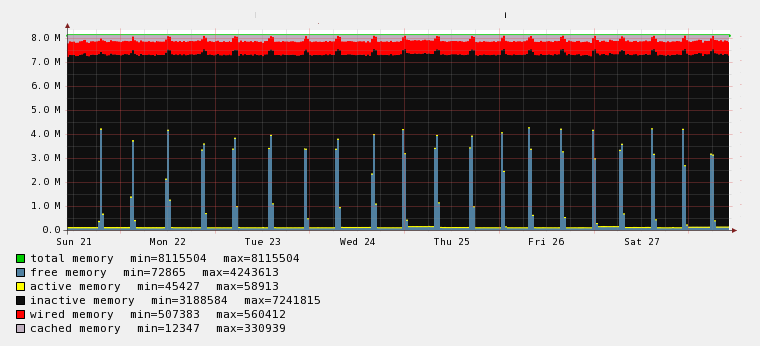
\includegraphics[scale=0.36]{pics/memory-7day.eps} \\
\end{center}

\subsection{Know your systems.}
CPU load - 30 days
\begin{center}
	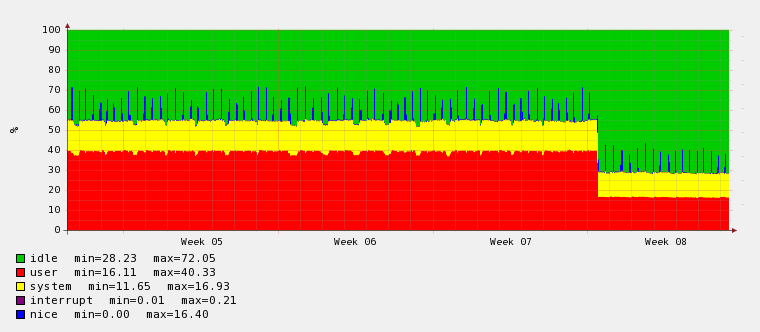
\includegraphics[scale=0.9]{pics/cpu-30day.eps}
\end{center}

\subsection{Know your systems.}
30 days
\begin{center}
	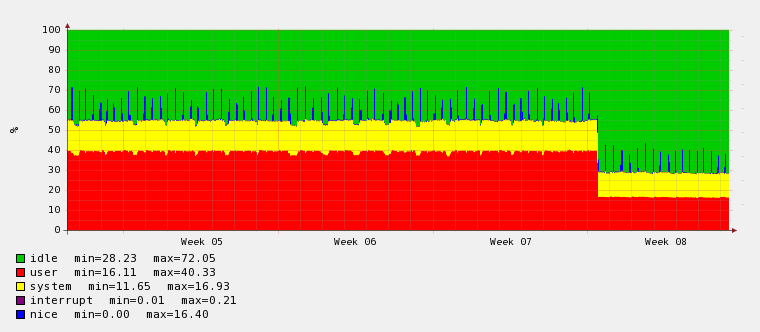
\includegraphics[scale=0.36]{pics/cpu-30day.eps}
	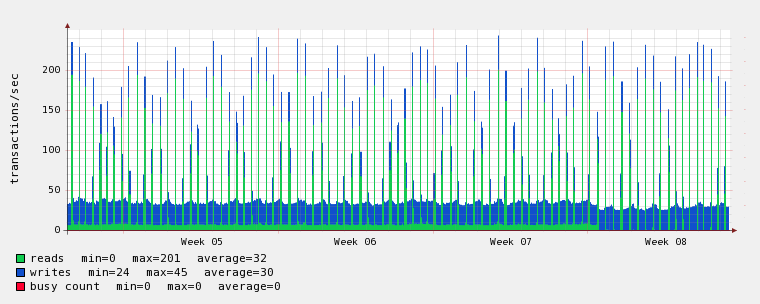
\includegraphics[scale=0.36]{pics/disk-io-30day.eps} \\
	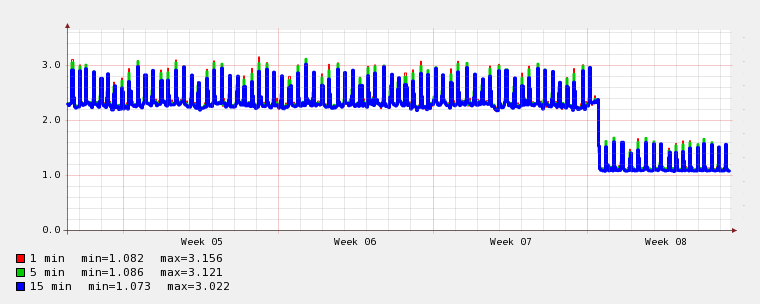
\includegraphics[scale=0.36]{pics/load-average-30day.eps}
	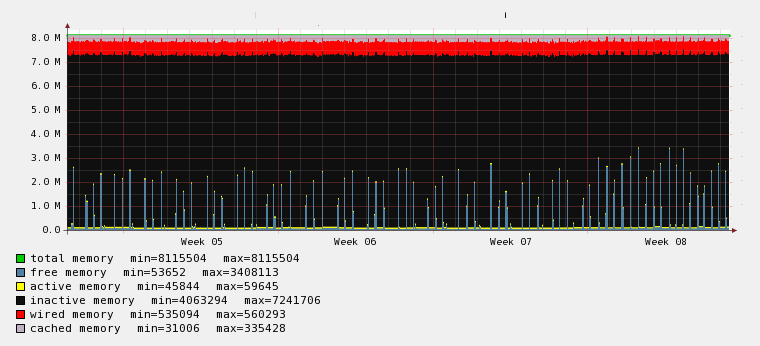
\includegraphics[scale=0.36]{pics/memory-30day.eps} \\
\end{center}

\subsection{Turn {\em events} into {\em metrics.}}
\begin{itemize}
	\item Log it!
\end{itemize}

\addvspace{.5in}
\begin{itemize}
	\item Export counters/timers from within your application.
	\item Process logs and produce counters/timers:
\begin{verbatim}
awk ’{print $9}’ /var/log/httpd/access.log | sort | uniq -c
\end{verbatim}
\end{itemize}

\addvspace{.5in}
\begin{itemize}
	\item Graph it. \\
	{\tt https://is.gd/tDCmQI}
\end{itemize}

\subsection{Monitoring/graphing}
SNMP based:
\begin{itemize}
	\item Cacti: \verb+http://www.cacti.net/+
	\item MRTG: \verb+http://oss.oetiker.ch/mrtg/+
	\item Observium: \verb+http://demo.observium.org/+
	\item ...
\end{itemize}
\vspace{.2in}
Other / complementary:
\begin{itemize}
	\item Ganglia: \verb+http://monitor.millennium.berkeley.edu/+
	\item Munin: \verb+http://munin.ping.uio.no/+
	\item Nagios: \verb+http://nagioscore.demos.nagios.com/+
	\item Graphite: \verb+http://graphite.wikidot.com/+
\end{itemize}
\vspace{.5in}
%More on monitoring and performance in a future lecture (if time permits).

\subsection{To the cloud!}
There’s a service for that. In the cloud. \\

Consider:
\begin{itemize}
	\item support / convenience vs. do-it-yourself
	\item integration with your other services
	\item data confidentiality
	\item data lock-in (esp. when trending data over years)
\end{itemize}

\subsection{Monitoring Pitfalls}
\vspace*{\fill}
\Huge
\begin{center}
Increasing the size of your haystack does not always
help in finding the needle.
\end{center}
\Normalsize
\vspace*{\fill}

\subsection{Monitoring Pitfalls}
\vspace*{\fill}
\Huge
\begin{center}
Increasing the size of your haystack does not always
help in finding the needle. \\
\vspace{.4in}
Email is not a scalable network monitoring solution.
\end{center}
\Normalsize
\vspace*{\fill}

\subsection{Monitoring Pitfalls}
\vspace*{\fill}
\Huge
\begin{center}
Increasing the size of your haystack does not always
help in finding the needle. \\
\vspace{.4in}
Email is not a scalable network monitoring solution. \\
\vspace{.4in}
Absence of a signal can itself be a signal.
\end{center}
\Normalsize
\vspace*{\fill}

\subsection{Monitoring Pitfalls}
\vspace*{\fill}
\Huge
\begin{center}
Increasing the size of your haystack does not always
help in finding the needle. \\
\vspace{.4in}
Email is not a scalable network monitoring solution. \\
\vspace{.4in}
Absence of a signal can itself be a signal. \\
\vspace{.4in}
This list is incomplete.
\end{center}
\Normalsize
\vspace*{\fill}

\subsection{Reading}
Hurricane Sandy
\begin{itemize}
	\item \verb+http://is.gd/aaxzvI+
	\item \verb+http://is.gd/Y75pEA+
	\item \verb+http://is.gd/32Az7y+
	\item \verb+http://is.gd/FhAuFZ+
\end{itemize}

\subsection{Reading}
Backups with {\tt dump(8)} and {\tt restore(8)}:
\begin{itemize}
	\item \verb+dump(8)+ and \verb+restore(8)+
	\item \verb+https://is.gd/bXG9of+
\end{itemize}
\vspace{.5in}

Filesystem snapshots:
\begin{itemize}
	\item \verb+https://en.wikipedia.org/wiki/Snapshot_(computer_storage)+
	\item \verb+https://en.wikipedia.org/wiki/Time_Machine_(Apple_software)+
	\item \verb+http://comet.lehman.cuny.edu/jung/cmp426697/WAFL.pdf+
\end{itemize}
\vspace{.5in}
Book: \verb+http://www.oreilly.com/catalog/unixbr/+



\subsection{Reading}
% % SNMP:
% % \begin{itemize}
% % 	\item \verb+http://is.gd/1LwOSD+
% % 	\item RFCs 1157, 3411, 3418 and others
% % 	\item \verb+snmpcmd(1)+
% % \end{itemize}

Monitoring:
\begin{itemize}
	\item {\tt https://www.paperplanes.de/2013/3/28/monitoring-for-humans.html}
	\item {\tt https://monitorama.com}
	\item {\tt https://www.slac.stanford.edu/xorg/nmtf/nmtf-tools.html}
	\item {\tt https://www.datadoghq.com/}
	\item {\tt https://www.newrelic.com/}
	\item {\tt https://www.elastic.co/products/logstash}
	\item {\tt https://www.splunk.com/}
\end{itemize}

\end{document}
